
	\chapter{Architectural description}
		\section{Overview}
			\paragraph{}
				The product is a distributed application based on the three logic layers of
				\begin{quote}
					\begin{description}
						\item[Presentation] manages the user's interaction with the system
						\item[Application] handles the logic of the system
						\item[Data] manages the information.
					\end{description}
				\end{quote}				 
			\paragraph{}
				Those three layers are divided onto four different physical tiers. As shown in \ref{fig:tiers}, Presentation and Data levels reside on a single tier, while Application level is split into two tiers (Web Server and Application Server). The Web Server is in charge of serving static assets and of forwarding API requests to the Application Server, which in turn implements the business logic of the application.
				\begin{figure}[!h]
					\centering
					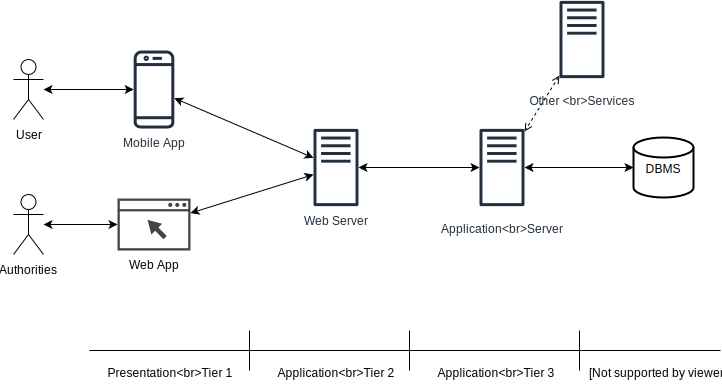
\includegraphics[width=\textwidth]{images/DD2/SimplifiedDeploymentView.pdf}
					\caption{Layers and tiers diagram}
					\label{fig:tiers}
				\end{figure}
			\paragraph{}
				In order to maximize the scalability of the system, both the Web and Application servers follow a scale-out approach: performances improvement is obtained through nodes replication. Because of this approach, load-balancing system are used in order to distribute the working load among the various nodes. 
				
				All the nodes of the Application Server use a "share everything" configuration, because there is only one shared database with one point of access. 
				
				Moreover, the Data layer is accomplished by exploiting an external DBMS service already available on the market. In this way we avoid devoting time on difficult problems about data replication and consistency, which are already solved by the existing and well tested database systems.
			\paragraph{}
				Every communication channel is secured by using firewalls. In this way, the Web Server is secured in a DMZ while Application Server protected as part of the LAN, so attacks and intrusions from malicious  clients will be prevented. It is important to note that, because the DBMS is located on a different tier with respect to the Application Server, a firewall between them can improve the security of the system.
				
				Finally, communication channels between the Application server and other services, like the Ticket Service, are secured for the same reasons explained above.
				\begin{figure}[!h]
					\centering
					\includegraphics[width=\textwidth]{images/DD2/SystemArchitecture.pdf}
					\caption{System architecture}
				\end{figure}
		\clearpage
		\section{Component view}
			\begin{figure}[!h]
				\centering
				\includegraphics[width=\textwidth]{images/DD2/ComponentDiagram.pdf}
				\caption{Component view diagram}
			\end{figure}
			\paragraph{}
				The Component view diagram represents, explicitly, only the components of the Application server, as they depict the main section of the system. 
				Below, is describe in depth the function of every internal server component made ad-hoc for the system (the ones in green).
			\begin{description}
				\item[Router]: receives HTTP over SSL/TLS requests following the REST paradigm (see also \ref{sez:componentInterface}) and forwards them to the others internal components of the Application server. Then, it forwards the replies back to the clients. It is relevant to note that temporary tokens are adopted, in order to define which functionalities are accessible for each client. Every client receives its personal token after the login procedure. 
				\item[UserManager]: 
					\begin{itemize}
						\item \textbf{LoginManager}: this component is responsible for granting access to registered users. In particular, the component receives the access credentials and, if they are correct, it returns a unique token used for further communication by the user. otherwise it returns an error message
						\item \textbf{SignUpManager}:  this component is responsible for the registration of unregistered users. In particular it receives the new access credentials and, if they are acceptable, it saves them in the system's database, otherwise it returns an error message
					\end{itemize}
				\item[ReportManager]: 
					\begin{itemize}
						\item \textbf{ReportReceiver}: this component is responsible for receiving the data of new reports and storing them in the database. In particular it takes care of the following tasks:
							\begin{itemize}
								\item employ the MS APIs to retrieve the information about which municipality the report has been created from
								\item recognizing the vehicle's plate in the picture, by employing the OCRS APIs. In case of an unrecognizable plate, the report status will be set to "NOT VALID" by default and a NULL vehicle will be set, otherwise it will be "NOT VERIFIED" (which means that a Local Officer has still to prove its validity) and the correct vehicle is associated to the report
								\item saving the report in the system's database
							\end{itemize}
						\item \textbf{ReportValidator}: this component is responsible for two main operations:
							\begin{itemize}
								\item fetching, from the database, of reports with status set to "NOT VERIFIED"
								\item  modification of status of a set of report, by changing it from "NOT VERIFIED" to "VALID" or "NOT VALID" according to the request sent by the local officer. Then it saves them in the database and sends them to the TS (if set to "VALID"), responsible for issuing traffic tickets
							\end{itemize}
					\end{itemize}
				\item[ReportMiner]: this component is responsible for obtaining reports by querying the database. It is crucial to note that the request can come directly from the Router or from other components like the ImprovementsManager and StatisticsComputationManager. In both cases, the municipality (obtained by the authority requiring or from the position required) is used for filtering reports. Only reports with status set to "VALID" are fetched. Various form of mining can be performed, in particular it's is possible to mine:
					\begin{itemize}
						\item All: all the reports produced in the specific municipality, are returned
						\item By Type: between all the reports produced in the specific municipality only those which have the given violation's type are returned 
						\item By Date: between all the reports produced in the specific municipality only those which were composed on the given date are returned
						\item By Time: between all the reports produced in the specific municipality only those which were composed on the given time, regardless the date, are returned
						\item By Area: between all the reports produced in the specific municipality only those which were composed in the given area, defined by a center and a radius, are returned
					\end{itemize}
				In each case, if there are no reports satisfying the request, an error message is returned.
				\item[ImprovementManager]: this component is responsible for getting the possible improvements belonging to the requesting authority's municipality and for setting their status. In order to determine the possible improvements, it crosses the data coming from the external MAS and from the MineReports component. When a new improvement is determined, it's status is set by default to "NOT DONE" and it is saved in the database. When no further improvements can be discovered, all those which have the status set to "NOT DONE" are returned to the requester. Moreover, through this component, an authority can set the status of a specific improvement to "DONE", after fetching all the possible one as described before. 
				\item[StatisticsComputationManager]: this component is responsible for building statistics, belonging to the requesting authority's municipality, about the violations and the perpetrators who cause them, by crossing the information coming from reports received by the ReportMiner and from issued tickets coming from the TS. It is important to note that statistics are always crunched on request and never saved on the server, because they can change at any time.
				\item[StatisticsDownloadManager]:this component is responsible for creating a non-materialized document (which means it is not saved on server side, but only generated and sent) about the statistics, belonging to the requesting authority's municipality,  by fetching them from the StatisticsComputationManager. The resulting document is returned to the caller
			\end{description}
		\section{Deployment view}
			\begin{figure}[!h]
				\centering
				\includegraphics[width=\textwidth]{images/DD2/DeploymentView.pdf}
				\caption{Deployment view diagram}
			\end{figure}
			\paragraph{}
				This picture shows how the system should be deployed (ignoring external services):
				\begin{itemize}
					\item It is available for end users as a Mobile Application, while, for authorities, as a Web Application, accessible both from Mobile and PC (using a browser)
					\item The Web Server, deployed on its physical node, has the purpose of serving static assets without intervention by the Application Server. Any other request received from the clients (both the Web and Mobile application) is automatically forwarded to the Application Server
					\item The Application Server and the Database Server are deployed on two different physical nodes, in order to have more security for data and to achieve a decoupled architecture
				\end{itemize}
		\section{Runtime view}
			\paragraph{}
				This section contains the most important RuntimeView, organized by the previous depicted UseCases (see RASD document).
				
				In order to simplify the complexity of those diagrams, we decided to describe in separate diagrams cases of access errors (which happen when the provided token does not authorize the requested operation), database's access errors and direct reply from the WebServer (the WebServer forwards every request, but in case of static contents request, it can reply directly without contacting the router if it has cached the content).
			\subsection{Registered User}
				\subsubsection{Add report}
					\begin{figure}[!h]
						\centering
						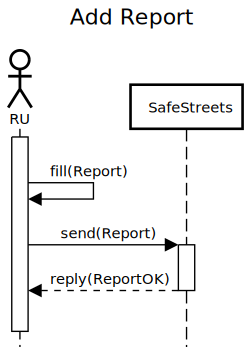
\includegraphics[width=\textwidth]{images/DD2/RuntimeView/RU/AddReport.pdf}
						\caption{Add report runtime view diagram}
					\end{figure}
					\paragraph{}
						In this sequence diagram the process through which a RU adds a report to the system is shown. 
						
						At first the RU chooses the "Add report" functionality on the UserMobileApp and composes the report. The app fetches a map from the MS and forwards the request to the Web Server, which contacts the Router. The Router forwards the request to the ReportReceiver, which tries to recognize the plate with the help of the OCRS, gets the municipality where the report has been issued through the MS and, finally, adds the report to the database through the DBMS.
				\subsubsection{Get my reports}
					\begin{figure}[!h]
						\centering
						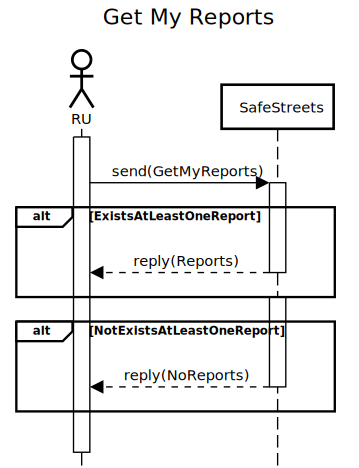
\includegraphics[width=\textwidth]{images/DD2/RuntimeView/RU/GetMyReports.pdf}
						\caption{Get my reports runtime view diagram}
					\end{figure}
					\paragraph{}
						In this sequence diagram the process through which a RU gets all the reports he/she has issued is shown.
						
						At first the RU chooses the "Get my reports" functionality on the UserMobileApp. Then the app starts fetching all the reports issued by the user. In particular, every request passes through the WebServer, Router, ReportMiner and finally the DBMS, then it goes back to the UserMobileApp. Once all the reports have been fetched, they are presented to the RU.
				\clearpage
				\subsubsection{Get unsafe areas}
					\begin{figure}[!h]
						\centering
						\includegraphics[width=\textwidth]{images/DD2/RuntimeView/RU/GetUnsafeAreas.pdf}
						\caption{Get unsafe areas runtime view diagram}
					\end{figure}
					\paragraph{}
						In this sequence diagram is displayed the process which permits a RU to discover all the types, dates and times of reports issued in a selected area. 
						
						This starts with the request, by the RU, that gets sent to the Web Server which will forward it to the Router. The Router will call "getUnsafeAreas" on the ReportMiner component that will query the database. When the response is ready it will go back through the same path.
			\clearpage
			\subsection{Authority}
				\subsubsection{Get statistics}
					\begin{figure}[!h]
						\centering
						\includegraphics[width=\textwidth]{images/DD2/RuntimeView/Authority/GetStatistics.pdf}
						\caption{Get statistics runtime view diagram}
					\end{figure}
					\paragraph{}
						In this sequence diagram the request gets sent to the WebServer and forwarded to the Router. Here, the StatisticsComputationManager is called. This component requests tickets data from the TS and then uses the ReportMiner component to access the database. If there are enough data, the StatisticsComputationManager generates new statistics. If the request from the authority was to only visualize the statistics, the StaticsComputationManager will send them back to the Router and to the authority, otherwise, by starting a new request, the StatisticsDownloadManager asks the StaticsComputationManager for new statistics, creates a non-materalized document and sends it back through the Router.
				\clearpage
				\subsubsection{Mine reports}
					\begin{figure}[!h]
						\centering
						\includegraphics[width=\textwidth]{images/DD2/RuntimeView/Authority/MineReports.pdf}
						\caption{Mine reports runtime view diagram}
					\end{figure}
					\paragraph{}
						This sequence diagram shows how the authorities can mine the reports. 
						
						At first all the reports in the authority's municipality are fetched through the following procedure. The mine request gets sent from the Web App to the Web Server which sends it forward to the Router. The ReportMiner gets called, it queries the database and, if enough reports are found, the list containing them is created and sent back to Web App. When there are less reports than needed, an error message will reach the authority. When the Web App receives the list of reports, it uses the MS to display them. 
						
						Now the requester is able to decide a filter to the search, choosing between the ones described in the ReportMiner component description. In order to fetch the filtered reports, the same procedure described before is used, but the requestType will be different from "ALL".
			\clearpage
			\subsection{Local Officer}
				\subsubsection{Validate reports}
					\begin{figure}[!h]
						\centering
						\includegraphics[width=\textwidth]{images/DD2/RuntimeView/Authority/LO/ValidateReports.pdf}
						\caption{Validate reports runtime view diagram}
					\end{figure}
					\paragraph{}
						The request gets sent with the standard route until the ReportValidator gets reached. Report validator queries the DBMS for reports to be validated, if there are none an error message is shown back to the Web App, otherwise the reports are sent back to the Web App, where they are displayed also thanks to of the MS.
						The LO can at this point start to validate the reports. When a report gets validated, with any result of validation, it gets sent back to the ReportValidator component which updates the database and, if the report is set as "VALID", it is also sent to the TS with a POST request. The process continues until the LO stops to validate reports.
			\clearpage
			\subsection{Municipal Employee}
				\subsubsection{Get improvements}
					\begin{figure}[!h]
						\centering
						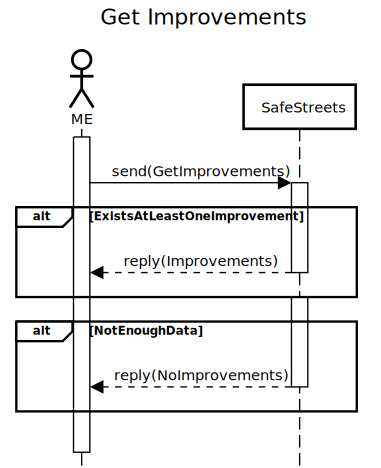
\includegraphics[width=\textwidth]{images/DD2/RuntimeView/Authority/ME/GetImprovements.pdf}
						\caption{Get improvements runtime view diagram}
					\end{figure}
					\paragraph{}
						This sequence diagram shows the request of improvements from a ME. 
						
						Using the standard route, the request reaches the ImprovementManager, which gets from the MAS, through a GET request, the list of accidents that took place in the ME's municipality. The ReportMiner then is tasked to obtain, from the DBMS, the list of reports of the Municipality, retuning them, in case of success or returning an error to the Web App, in case of failure. 
						
						With the data received from the MAS and the ReportMiner, the ImprovementManager computes all possible improvements that, in a loop, are sent and memorized by the DBMS only if they were not already present. Finished the update, the ImprovementManager retrieves from the database, using the "retrieveImprovements" function, all possible "NOT DONE" improvements for the ME's municipality. The list of improvements is then sent back through the Router to the Web App where the ME can visualize and eventually set them as "DONE". 
						
						When at least one improvement gets its status changed, the Web App sends a request back to the Web Server and the Router. The ImprovementManager is then called by the Router to update the status of the improvement on the database.
			\subsection{Extra cases}
				\subsubsection{Database access error}
					\begin{figure}[!h]
						\centering
						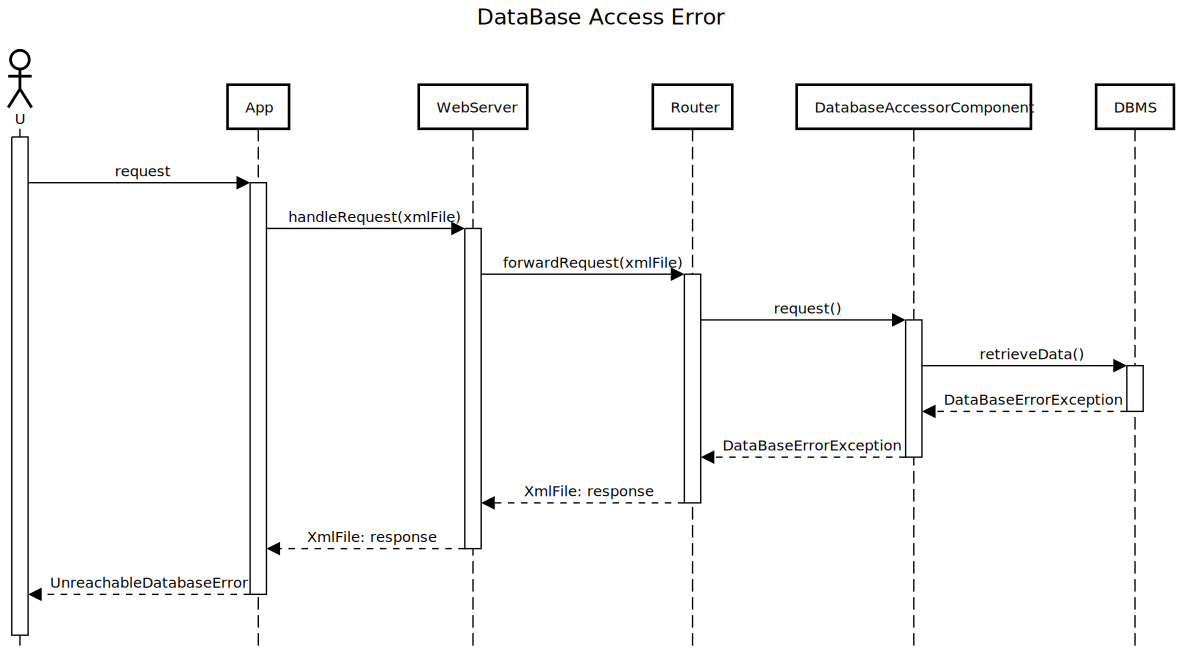
\includegraphics[width=\textwidth]{images/DD2/RuntimeView/Error/dbAccessError.pdf}
						\caption{Database access error runtime view diagram}
					\end{figure}
					\paragraph{}
						In this case a user U (which can be a RU, ME or LO) tries to use a functionality that accesses the database, but the database is not accessible.
				\clearpage
				\subsubsection{Invalid token}
					\begin{figure}[!h]
						\centering
						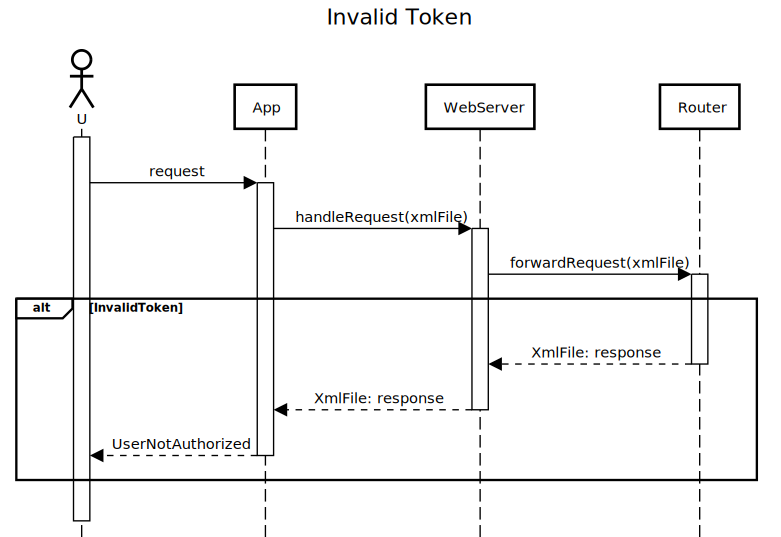
\includegraphics[width=0.6\textwidth]{images/DD2/RuntimeView/Error/invalidToken.pdf}
						\caption{Invalid token runtime view diagram}
					\end{figure}
					\paragraph{}
						In this case a user U (which can be a RU, ME or LO) tries to use a functionality that is not accessible with the given token (for example a RU that tries to MineReport).
		\section{Component interfaces}
			\paragraph{}
				The following picture contains all the used interface in the system.
				\begin{figure}[!h]
					\centering
					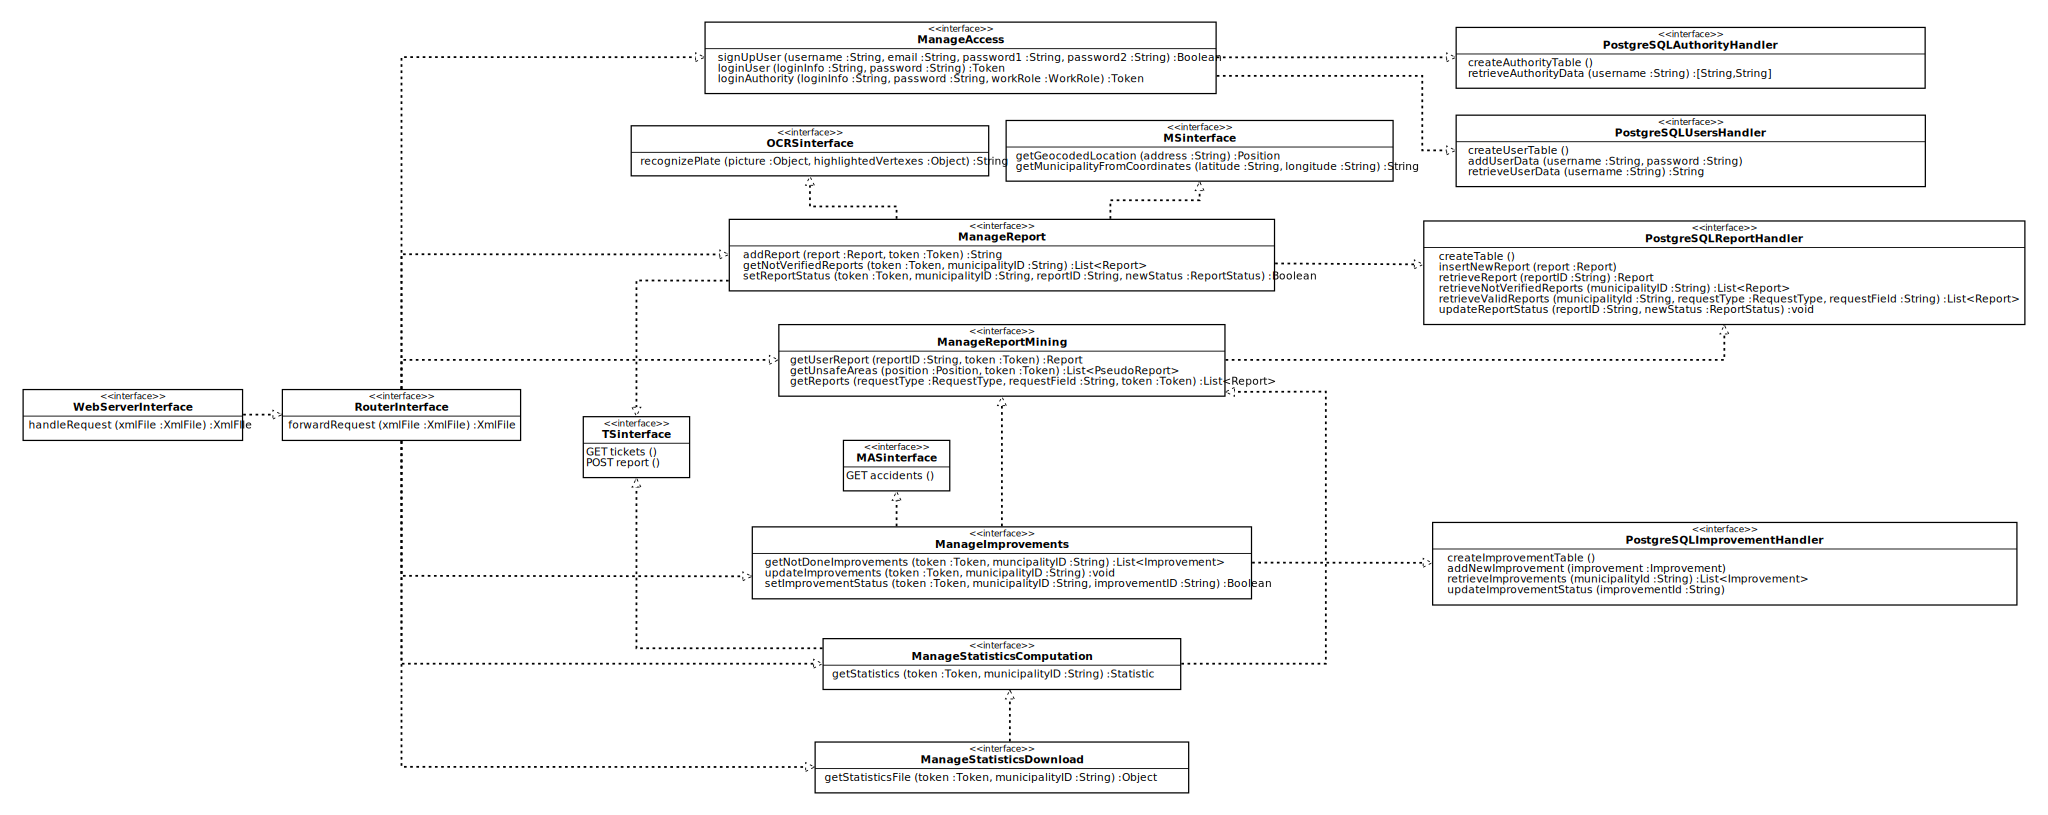
\includegraphics[width=\textwidth]{images/DD2/interfaces.pdf}
					\caption{Component interfaces}
				\end{figure}
			\paragraph{}
				As the development continued, the class diagram introduced in the RASD document has been updated. So we decided to  report here the new version, with classes used by the interfaces described below.
				\begin{figure}[!h]
					\centering
					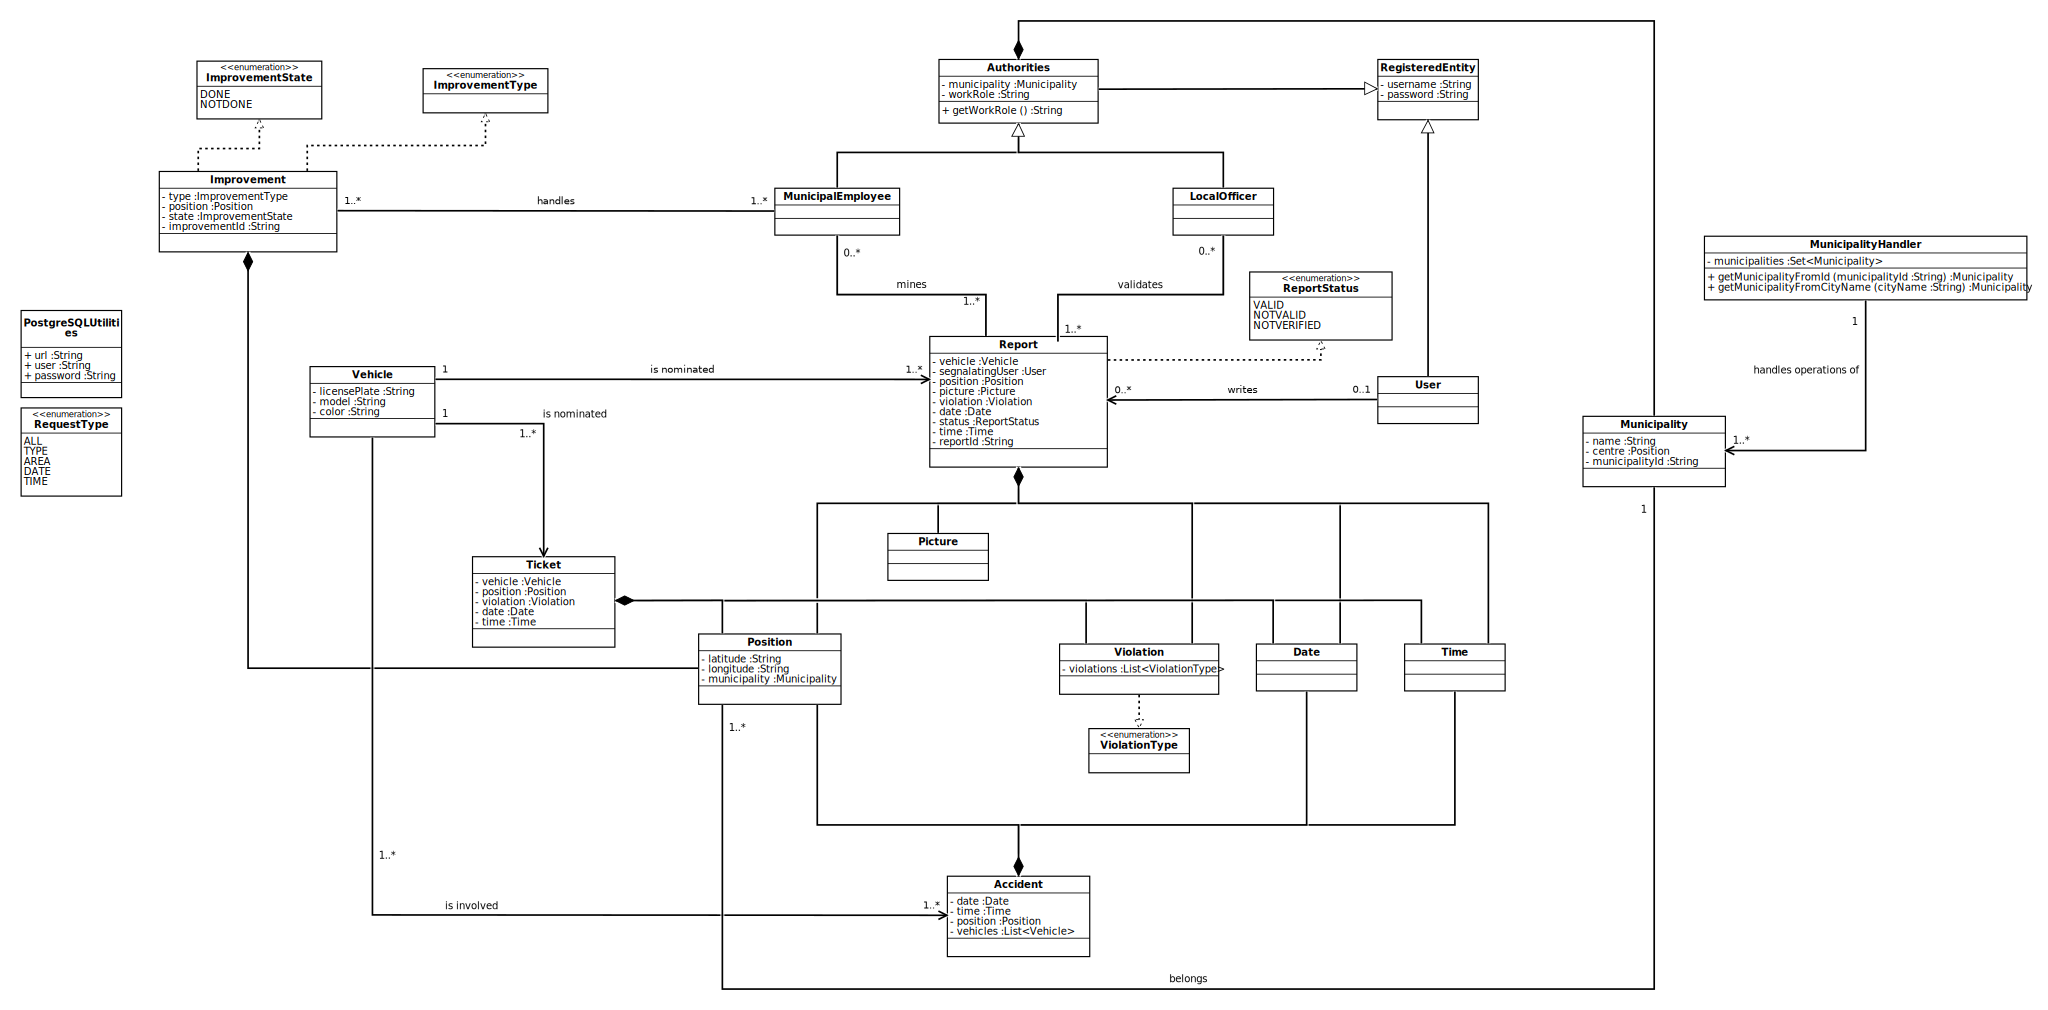
\includegraphics[width=\textwidth]{images/DD2/classDiagram.pdf}
					\caption{Class diagram}
				\end{figure}
			\newpage
			\subsection{Web Server interface and Report interface}
				\paragraph{}
					For the Web server interface and the Report interface a RESTful API has been chosen. Since both interfaces are a vital part of the system and the components that they connect belongs to the part that will be implemented, they will be discussed in depth.
				\subsubsection{REST table of resources}
					\paragraph{}
						The following table represents the logic structures of the resources of the system and the operation that can be done on them.
						\begin{table}[!h]
							\centering
							\begin{tabular}{lcccc}
								\toprule
								\textbf{URI}	& \textbf{POST} & \textbf{GET} & \textbf{PUT} & \textbf{DELETE} \\
								\midrule
								/users/registration/?id=xxx & X & - & - & - \\
								/users/login/?id=xxx & - & X & - & - \\
								/users/authorities/login/?id=xxx & - & X & - & - \\
								/reports/default & X & - & - & - \\
								/reports/default/?id=xxx & - & X & - & - \\
								/reports/default/unsafearea & - & X & - & - \\
								/reports/notverified/?id=xxx & - & X & X & - \\
								/reports/valid/?id=xxx & - & X & - & - \\
								/improvements/?id=xxx & - & X & X & - \\
								/statistics/visualize/?id=xxx & - & X & - & - \\
								/statistics/download/?id=xxx & - & X & - & - \\
							\end{tabular}
							\caption{REST table of resources}
						\end{table}
					\paragraph{}
						"X" : the operation is applicable on the resource
						
						"-" : the operation is inapplicable on the resource
					\clearpage
					\paragraph{}
						Here a quick description of the resources group:
						\begin{itemize}
							\item \textit{\textbf{/users/*}} represents the information related to the users, in particular their account information
							\item \textit{\textbf{/reports/default/*}} represents the resources accessible by the RU, in particular reports and "pseudo report" for the unsafe areas. These resources will be greatly used by the mobile app.
							\item \textit{\textbf{/reports/notverified/*}} contains all the received reports that haven't been immediately discarded by the OCRS but are still on impending evaluation by a LO
							\item \textit{\textbf{/reports/valid/*}} contains all the received reports that have been judged as valid by a LO
							\item \textit{\textbf{/improvements/*}} contains the improvements suggested to a municipality that can be retrieved by a ME
							\item \textit{\textbf{/statistics/*}} contains the statistics that can be retrieved by an authority
						\end{itemize}
				\subsubsection{General request description}
					\paragraph{}
						The data that will be transmitted will be composed of XML files.
						
						To recognize the user who sent a request to the server, the system will employ tokens. A token is a string that is provided to the user as an answer to the login, it contains information on the user and will always be part of the requests, except the login and sign up.
						The contained information will be:
						\begin{itemize}
							\item User type information: the different type users (RU, LO and ME) will be identified in different ways to avoid ambiguity. Moreover the identifier for LO and ME will contain an identifier for the Municipality they work for
							\item User identifier: The single user will be identified to have information on who is making the request and give the correct permission to access data.
							\item Creation time: The token is a "one time only" use. Its validity is fixed and will generally last at least for a session, this permits to recycle pieces of tokens and avoids the malicious use of old ones to get data.
						\end{itemize}
				\subsubsection{Detailed requests}
					\paragraph{}
						\textbf{POST} /users/registration/?id={id}
						
						This request is used to register a user
					\paragraph{}
						\textbf{Parameters}
						\begin{table}[!h]
							\begin{tabular}{L{0.2\textwidth}L{0.2\textwidth}L{0.4\textwidth}}
								\toprule
								Field & Type & Description \\
								\midrule
								 id & String & The username of the user who is trying to register \\
								 \bottomrule
							\end{tabular}
						\end{table}
					\clearpage
					\paragraph{}
						\textbf{Fields}
						\begin{table}[!h]
							\begin{tabular}{L{0.25\textwidth}L{0.15\textwidth}L{0.4\textwidth}}
								\toprule
								Field & Type & Description \\
								\midrule
								 email & String & The email of the user \\
								 passwordFirst & String & The password of the user \\
								 passwordSecond & String & The same password as before, used to confirm the first password \\
								 \bottomrule
							\end{tabular}
						\end{table}
					\paragraph{}
						\textbf{Success 201} (resource created)
					\paragraph{}
						\textbf{Error 401}
						\begin{table}[!h]
							\begin{tabular}{L{0.3\textwidth}L{0.5\textwidth}}
								\toprule
								Field & Description \\
								\midrule
								 ExistingUsername & Someone with the same username is already registered \\
								 DifferentPassword & The second password is different from the first one \\
								 ExistingMail & This email is already associated with another account \\
								 \bottomrule
							\end{tabular}
						\end{table}
						
						\paragraph{}
						\textbf{GET} /users/login/?id={id}
						
						This request allows a RU to login
						\paragraph{}
							\textbf{Parameters}
							\begin{table}[!h]
								\begin{tabular}{L{0.2\textwidth}L{0.2\textwidth}L{0.4\textwidth}}
									\toprule
									Field & Type & Description \\
									\midrule
								 	id & String & The username of the user who is trying to login \\
								 	\bottomrule
								\end{tabular}
							\end{table}
						\paragraph{}
							\textbf{Fields}
							\begin{table}[!h]
								\begin{tabular}{L{0.25\textwidth}L{0.15\textwidth}L{0.4\textwidth}}
									\toprule
									Field & Type & Description \\
									\midrule
								 	loginInformation & String & The email or username of the user \\
								 	password & String & The password of the user \\
								 	\bottomrule
								\end{tabular}
							\end{table}
						\clearpage
						\paragraph{}
							\textbf{Success 200} (request ok)
							\begin{table}[!h]
								\begin{tabular}{L{0.2\textwidth}L{0.2\textwidth}L{0.4\textwidth}}
									\toprule
									Field & Type & Description \\
									\midrule
									token & String & A token that represents the user \\
									reportIDs & String[] & The list of id associated with the reports uploaded by the user \\
								 	\bottomrule
								\end{tabular}
							\end{table}
						\paragraph{}
							\textbf{Error 401} (Unauthorized)
							\begin{table}[!h]
								\begin{tabular}{L{0.4\textwidth}L{0.4\textwidth}}
									\toprule
									Field & Description \\
									\midrule
								  	WrongUsernameOrPassword & The written username and password does not correspond to any existing user \\
								 	\bottomrule
								\end{tabular}
							\end{table}
							
						\paragraph{}
						\textbf{GET} /users/authorities/login/?id={id}
						
						This request allows a ME or LO to login
						\paragraph{}
							\textbf{Parameters}
							\begin{table}[!h]
								\begin{tabular}{L{0.2\textwidth}L{0.2\textwidth}L{0.4\textwidth}}
									\toprule
									Field & Type & Description \\
									\midrule
								 	id & String & The username of the user who is trying to login \\
								 	\bottomrule
								\end{tabular}
							\end{table}
						\paragraph{}
							\textbf{Fields}
							\begin{table}[!h]
								\begin{tabular}{L{0.25\textwidth}L{0.15\textwidth}L{0.4\textwidth}}
									\toprule
									Field & Type & Description \\
									\midrule
								 	loginInformation & String  & The username of the user \\
								 	password & String & The password of the user \\
								 	workRole & String & This will be 'ME' or 'LO' \\
								 	\bottomrule
								\end{tabular}
							\end{table}
						\paragraph{}
							\textbf{Success 200} (request ok)
							\begin{table}[!h]
								\begin{tabular}{L{0.25\textwidth}L{0.1\textwidth}L{0.45\textwidth}}
									\toprule
									Field & Type & Description \\
									\midrule
									token & String & A token that represents the user and the municipality he/she works in \\
									municipalityID & String & The id of the municipality where the ME or LO works, this will be a parameter for the following requests \\
								 	\bottomrule
								\end{tabular}
							\end{table}
						\clearpage
						\paragraph{}
							\textbf{Error 401} (Unauthorized)
							\begin{table}[!h]
								\begin{tabular}{L{0.4\textwidth}L{0.4\textwidth}}
									\toprule
									Field & Description \\
									\midrule
								  	WrongUsernameOrPassword & The written username and password does not correspond to any existing user \\
								  	NotCorrespondingRole & The selected work role does not correspond to the user which given login and password corresponds to \\
								 	\bottomrule
								\end{tabular}
							\end{table}
							
						\paragraph{}
						\textbf{POST} /reports/default
						
						This request adds a report to the system
						\paragraph{}
							\textbf{Fields}
							\begin{table}[!h]
								\begin{tabular}{L{0.23\textwidth}L{0.15\textwidth}L{0.42\textwidth}}
									\toprule
									Field & Type & Description \\
									\midrule
								 	vehicle & Object & The vehicle information \\
								 	\hspace{2.5mm}licensePlate & String & The license plate of the vehicle \\
								 	position & Object & The position, expressed in DMS, of the vehicle when the report was submitted  \\
								 	\hspace{2.5mm}latitude & String & The latitude where the vehicle was recorded to be \\
								 	\hspace{3mm}longitude & String & The longitude where the vehicle was recorded to be \\
								 	picture & Object & Representation of the image of the vehicle \\
								 	violation & Object[] & An array of the type of violation \\
								 	\hspace{2.5mm}violationType & String & The type of violation \\
								 	date & String & The datetime in \newline dd-MM-yyyyThh:mm:ss format \\
								 	highlightVertexes & Object & The coordinates on the picture of where the license plate is located \\
								 	\hspace{2.5mm}vertexOne & Number[] & The coordinates (on the picure) of the top-left vertex \\
								 	\hspace{2.5mm}vertexTwo & Number[] & The coordinates (on the picture) of the bottom-right vertex \\
								 	\bottomrule
								\end{tabular}
							\end{table}
						\clearpage
						\paragraph{}
							\textbf{Success 201} (resource created)
							\begin{table}[!h]
								\begin{tabular}{L{0.2\textwidth}L{0.2\textwidth}L{0.4\textwidth}}
									\toprule
									Field & Type & Description \\
									\midrule
									id & String & The id that the system has assigned to the sent report. This id will uniquely identify the report and will also contain information about the user which sent it\\
								 	\bottomrule
								\end{tabular}
							\end{table}
						
						\paragraph{}
						\textbf{GET} /reports/default/?id={id}
						
						This request retrieves a report form the system.
						\paragraph{}
							\textbf{Parameters}
							\begin{table}[!h]
								\begin{tabular}{L{0.2\textwidth}L{0.2\textwidth}L{0.4\textwidth}}
									\toprule
									Field & Type & Description \\
									\midrule
								 	id & String & The id that uniquely identifies the report that the user wants to see \\
								 	\bottomrule
								\end{tabular}
							\end{table}
						\paragraph{}
							\textbf{Success 200} (request ok)
							\begin{table}[!h]
								\begin{tabular}{L{0.23\textwidth}L{0.15\textwidth}L{0.42\textwidth}}
									\toprule
									Field & Type & Description \\
									\midrule
								 	vehicle & Object & The vehicle information \\
								 	\hspace{2.5mm}licensePlate & String & The license plate of the vehicle \\
								 	position & Object & The position, expressed in DMS, of the vehicle when the report was submitted  \\
								 	\hspace{2.5mm}latitude & String & The latitude where the vehicle was recorded to be \\
								 	\hspace{3mm}longitude & String & The longitude where the vehicle was recorded to be \\
								 	picture & Object & Representation of the image of the vehicle \\
								 	violation & Object[] & An array of the type of violation \\
								 	\hspace{2.5mm}violationType & String & The type of violation \\
								 	date & String & The datetime in \newline dd-MM-yyyyThh:mm:ss format \\
								 	highlightVertexes & Object & The coordinates on the picture of where the license plate is located \\
								 	\hspace{2.5mm}vertexOne & Number[] & The coordinates (on the picure) of the top-left vertex \\
								 	\hspace{2.5mm}vertexTwo & Number[] & The coordinates (on the picture) of the bottom-right vertex \\
								 	\bottomrule
								\end{tabular}
							\end{table}
						\paragraph{}
							\textbf{Error 403} (Forbidden)
							\begin{table}[!h]
								\begin{tabular}{L{0.4\textwidth}L{0.4\textwidth}}
									\toprule
									Field & Description \\
									\midrule
								  	 NoReportError & The requested resource caused an error on the database, this could both mean that the resource was not found on the database or that the database had internal error or an error on the connection \\
								 	\bottomrule
								\end{tabular}
							\end{table}
	
						\paragraph{}
						\textbf{GET} /reports/default/unsafearea
						
						This request retrieves the type of violations in certain area
						\paragraph{}
							\textbf{Fields}
							\begin{table}[!h]
								\begin{tabular}{L{0.23\textwidth}L{0.15\textwidth}L{0.42\textwidth}}
									\toprule
									Field & Type & Description \\
									\midrule
								 	 position & Object & The position, expressed in DMS, of the center of the area which the RU wants to know about \\
								 	 \hspace{2.5mm} latitude & String & The latitude where the vehicle was recorded to be \\
								 	 \hspace{2.5mm} longitude & String & The longitude where the vehicle was recorded to be \\
								 	\bottomrule
								\end{tabular}
							\end{table}
						\paragraph{}
							\textbf{Success 200} (request ok)
							\begin{table}[!h]
								\begin{tabular}{L{0.23\textwidth}L{0.15\textwidth}L{0.42\textwidth}}
									\toprule
									Field & Type & Description \\
									\midrule
									pseudoReport & Object[] & The list of partial reports that can be seen bya a RU \\
									\hspace{2.5mm} position & Object & The position, expressed in DMS, of the vehicle when the report was submitted  \\
									\hspace{5mm} latitude & String & The latitude where the vehicle was recorded to be \\
									\hspace{5mm} longitude & String & The longitude where the vehicle was recorded to be \\
									\hspace{2.5mm}violation & Object[] & An array of the type of violation \\
									\hspace{5mm}violationType & String & The type of violation  \\
								 	\bottomrule
								\end{tabular}
							\end{table}
						\clearpage
						\paragraph{}
							\textbf{Error 404} (Resource not found)
							\begin{table}[!h]
								\begin{tabular}{L{0.4\textwidth}L{0.4\textwidth}}
									\toprule
									Field & Description \\
									\midrule
								  	NoReportError & The requested resource caused an error on the database, this could both mean that the resource was not found on the database or that the database had internal error or an error on the connection \\
								 	\bottomrule
								\end{tabular}
							\end{table}
							
							\paragraph{}
						\textbf{GET} /reports/default/unsafearea
						
						This request retrieves the type of violations in certain area.
						\paragraph{}
							\textbf{Fields}
							\begin{table}[!h]
								\begin{tabular}{L{0.25\textwidth}L{0.15\textwidth}L{0.4\textwidth}}
									\toprule
									Field & Type & Description \\
									\midrule
								 	position & Object & The position, expressed in DMS, of the center of the area which the RU wants to know about \\
								 	\hspace{2.5mm}latitude & String & The latitude where the vehicle was recorded to be \\
								 	\hspace{2.5mm}longitude & String & The longitude where the vehicle was recorded to be \\
								 	\bottomrule
								\end{tabular}
							\end{table}
						\paragraph{}
							\textbf{Success 200} (request ok)
							\begin{table}[!h]
								\begin{tabular}{L{0.25\textwidth}L{0.1\textwidth}L{0.45\textwidth}}
									\toprule
									Field & Type & Description \\
									\midrule
									pseudoReport & Object[] & The list of partial reports that can be seen bya a RU \\
									\hspace{2.5mm}position & Object & The position, expressed in DMS, of the vehicle when the report was submitted  \\
									\hspace{5mm}latitude & String & The latitude where the vehicle was recorded to be \\
									\hspace{5mm}longitude & String & The longitude where the vehicle was recorded to be \\
									\hspace{2.5mm}violation & Object[] & An array of the type of violation \\
									\hspace{5mm}violationType & String & The type of violation \\
								 	\bottomrule
								\end{tabular}
							\end{table}
						\paragraph{}
							\textbf{Error 404} (Resource not found)
							\begin{table}[!h]
								\begin{tabular}{L{0.4\textwidth}L{0.4\textwidth}}
									\toprule
									Field & Description \\
									\midrule
								  	 NoReportError & The requested resource caused an error on the database, this could both mean that the resource was not found on the database or that the database had internal error or an error on the connection \\
								 	\bottomrule
								\end{tabular}
							\end{table}
						
						\paragraph{}
						\textbf{GET} /reports/notverified/?id={id}
						
						This request retrieves the reports that are waiting for validation in a certain municipality.
						\paragraph{}
							\textbf{Parameters}
							\begin{table}[!h]
								\begin{tabular}{L{0.2\textwidth}L{0.2\textwidth}L{0.4\textwidth}}
									\toprule
									Field & Type & Description \\
									\midrule
								 	id & String & The id that uniquely identifies the municipality which the LO works for \\
								 	\bottomrule
								\end{tabular}
							\end{table}
						\paragraph{}
							\textbf{Success 200} (request ok)
							\begin{table}[!h]
								\begin{tabular}{L{0.25\textwidth}L{0.1\textwidth}L{0.45\textwidth}}
									\toprule
									Field & Type & Description \\
									\midrule
									reports & Object[] & A list of the valid reports of a certain municipality \\
									\hspace{2.5mm}reportId & String & The string that uniquely identifies a report \\
									\hspace{2.5mm}vehicle & Object & The vehicle information \\
									\hspace{5mm}licensePlate & String & The license plate of the vehicle \\
									\hspace{2.5mm}position & Object & The position, expressed in DMS, of the vehicle when the report was submitted  \\
									\hspace{5mm}latitude & String & The latitude where the vehicle was recorded to be \\
									\hspace{5mm}longitude & String & The longitude where the vehicle was recorded to be \\
									\hspace{2.5mm}picture & Object & Representation of the image of the vehicle \\
									\hspace{2.5mm}violation & Object[] & An array of the type of violation \\
									\hspace{5mm}violationType & String & The type of violation \\
									\hspace{2.5mm}date & String & The datetime in \newline dd-MM-yyyyThh:mm:ss format \\
								 	\bottomrule
								\end{tabular}
							\end{table}
						\paragraph{}
							\textbf{Error 403} (Forbidden)
							\begin{table}[!h]
								\begin{tabular}{L{0.4\textwidth}L{0.4\textwidth}}
									\toprule
									Field & Description \\
									\midrule
								  	UserNotAuthorized & The id of the municipality and the token of the user have been analyzed. It was found that the user was not an LO or the LO's municipality was not the one of the reports requested \\
								 	\bottomrule
								\end{tabular}
							\end{table}
							
							\paragraph{}
						\textbf{PUT} /reports/notverified/?id={id}
						
						This request modifies the status of a report
						\paragraph{}
							\textbf{Parameters}
							\begin{table}[!h]
								\begin{tabular}{L{0.2\textwidth}L{0.2\textwidth}L{0.4\textwidth}}
									\toprule
									Field & Type & Description \\
									\midrule
								 	id & String & The id that uniquely identifies the municipality which the LO works for \\
								 	\bottomrule
								\end{tabular}
							\end{table}
						\paragraph{}
							\textbf{Fields}
							\begin{table}[!h]
								\begin{tabular}{L{0.25\textwidth}L{0.15\textwidth}L{0.4\textwidth}}
									\toprule
									Field & Type & Description \\
									\midrule
								 	id & String & The id of the report \\
								 	newStatus & String & The result of the validation performed by the LO \\
								 	\bottomrule
								\end{tabular}
							\end{table}
						\paragraph{}
							\textbf{Error 403} (Forbidden)
							\begin{table}[!h]
								\begin{tabular}{L{0.4\textwidth}L{0.4\textwidth}}
									\toprule
									Field & Description \\
									\midrule
								  	UserNotAuthorized & The id of the municipality and the token of the user have been analyzed. It was found that the user was not an LO or the LO's municipality was not the one of the reports requested \\
								 	\bottomrule
								\end{tabular}
							\end{table}
							
						\paragraph{}
						\textbf{GET} /reports/valid/?id={id}
						
						This request gets all the valid reports in a certain municipality.
						\paragraph{}
							\textbf{Parameters}
							\begin{table}[!h]
								\begin{tabular}{L{0.2\textwidth}L{0.2\textwidth}L{0.4\textwidth}}
									\toprule
									Field & Type & Description \\
									\midrule
								 	id & String & The id that uniquely identifies the municipality which the LO works for \\
								 	\bottomrule
								\end{tabular}
							\end{table}
						\paragraph{}
							\textbf{Fields}
							\begin{table}[!h]
								\begin{tabular}{L{0.25\textwidth}L{0.15\textwidth}L{0.4\textwidth}}
									\toprule
									Field & Type & Description \\
									\midrule
								 	requestType & String & The type of request issued (i.e. "by area") \\
								 	requestField & String & The field that contains precise information on the request \\
								 	\bottomrule
								\end{tabular}
							\end{table}
						\paragraph{}
							\textbf{Success 200} (request ok)
							\begin{table}[!h]
								\begin{tabular}{L{0.25\textwidth}L{0.1\textwidth}L{0.45\textwidth}}
									\toprule
									Field & Type & Description \\
									\midrule
									reports & Object[] & A list of the valid reports of a certain municipality \\
									\hspace{2.5mm}reportId & String & The string that uniquely identifies a report \\
									\hspace{2.5mm}vehicle & Object & The vehicle information \\
									\hspace{5mm}licensePlate & String & The license plate of the vehicle \\
									\hspace{2.5mm}position & Object & The position, expressed in DMS, of the vehicle when the report was submitted  \\
									\hspace{5mm}latitude & String & The latitude where the vehicle was recorded to be \\
									\hspace{5mm}longitude & String & The longitude where the vehicle was recorded to be \\
									\hspace{2.5mm}picture & Object & Representation of the image of the vehicle \\
									\hspace{2.5mm}violation & Object[] & An array of the type of violation \\
									\hspace{5mm}violationType & String & The type of violation \\
									\hspace{2.5mm}date & String & The datetime in \newline dd-MM-yyyyThh:mm:ss format \\
								 	\bottomrule
								\end{tabular}
							\end{table}
						\paragraph{}
							\textbf{Error 403} (Forbidden)
							\begin{table}[!h]
								\begin{tabular}{L{0.4\textwidth}L{0.4\textwidth}}
									\toprule
									Field & Description \\
									\midrule
								  	UserNotAuthorized & The id of the municipality and the token of the user have been analyzed. It was found that the user was not an LO or the LO's  municipality was not the one of the reports requested  \\
								 	\bottomrule
								\end{tabular}
							\end{table}
						\paragraph{}
							\textbf{Error 404} (Resource not found)
							\begin{table}[!h]
								\begin{tabular}{L{0.4\textwidth}L{0.4\textwidth}}
									\toprule
									Field & Description \\
									\midrule
								  	 NoReportError & The requested resource caused an error on the database, this could both mean that the resource was not found on the database or that the database had internal error or an error on the connection \\ 
								 	\bottomrule
								\end{tabular}
							\end{table}
							
						\paragraph{}
						\textbf{GET} /improvements/?id={id}
						
						This request retrieves all the suggested improvements in a certain municipality
						\paragraph{}
							\textbf{Parameters}
							\begin{table}[!h]
								\begin{tabular}{L{0.2\textwidth}L{0.2\textwidth}L{0.4\textwidth}}
									\toprule
									Field & Type & Description \\
									\midrule
								 	id & String & The id that uniquely identifies the municipality which the ME works for \\
								 	\bottomrule
								\end{tabular}
							\end{table}
						\paragraph{}
							\textbf{Success 200} (request ok)
							\begin{table}[!h]
								\begin{tabular}{L{0.25\textwidth}L{0.1\textwidth}L{0.45\textwidth}}
									\toprule
									Field & Type & Description \\
									\midrule
									improvements & Object[] & The list of suggested improvements \\
									\hspace{2.5mm}type & String & The of the improvement, i.e. "add a cycling lane" \\
									\hspace{2.5mm}position & Object & The position of the improvement expresses in DMS \
									\hspace{5mm}latitude & String & The latitude where the suggested improvement will be expected to be \\
									\hspace{5mm}longitude & String & The longitude where the suggested improvement will be expected to be  \\
									\hspace{2.5mm}state & String & The status of the improvement, it could be "DONE" or "NOT DONE" \\
									\hspace{2.5mm}improvementId & String & The id that uniquely identifies the improvement on the database \\
								 	\bottomrule
								\end{tabular}
							\end{table}
						\paragraph{}
							\textbf{Error 403} (Forbidden)
							\begin{table}[!h]
								\begin{tabular}{L{0.4\textwidth}L{0.4\textwidth}}
									\toprule
									Field & Description \\
									\midrule
								  	UserNotAuthorized & The id of the municipality and the token of the user have been analyzed. It was found that the user was not an ME or the ME's  municipality was not the one of the reports requested  \\
								 	\bottomrule
								\end{tabular}
							\end{table}
						\paragraph{}
							\textbf{Error 404} (Resource not found)
							\begin{table}[!h]
								\begin{tabular}{L{0.4\textwidth}L{0.4\textwidth}}
									\toprule
									Field & Description \\
									\midrule
								  	NotEnoughReportError & The requested improvements could not be found on the database and the available information on the Municipality is not enough to compute correct suggestions \\
								 	\bottomrule
								\end{tabular}
							\end{table}
						
						\paragraph{}
						\textbf{PUT} /improvements/?id={id}
						
						This request allows a ME or LO to login
						\paragraph{}
							\textbf{Parameters}
							\begin{table}[!h]
								\begin{tabular}{L{0.2\textwidth}L{0.2\textwidth}L{0.4\textwidth}}
									\toprule
									Field & Type & Description \\
									\midrule
								 	id & String & The id that uniquely identifies the municipality which the LO works for \\
								 	\bottomrule
								\end{tabular}
							\end{table}
						\paragraph{}
							\textbf{Fields}
							\begin{table}[!h]
								\begin{tabular}{L{0.25\textwidth}L{0.15\textwidth}L{0.4\textwidth}}
									\toprule
									Field & Type & Description \\
									\midrule
								 	improvementId & String & The id that uniquely identifies the improvement on the database \\
								 	\bottomrule
								\end{tabular}
							\end{table}
						\paragraph{}
							\textbf{Error 403} (Forbidden)
							\begin{table}[!h]
								\begin{tabular}{L{0.4\textwidth}L{0.4\textwidth}}
									\toprule
									Field & Description \\
									\midrule
								  	UserNotAuthorized & The id of the municipality and the token of the user have been analyzed. It was found that the user was not an ME or the ME's municipality was not the one of the reports requested \\
								 	\bottomrule
								\end{tabular}
							\end{table}
							
						\paragraph{}
						\textbf{GET} /statistics/visualize/?id={id}
						
						This request gets the available statistics on a certain municipality and lets the ME visualize them.
						\paragraph{}
							\textbf{Parameters}
							\begin{table}[!h]
								\begin{tabular}{L{0.2\textwidth}L{0.2\textwidth}L{0.4\textwidth}}
									\toprule
									Field & Type & Description \\
									\midrule
								 	id & String & The id that uniquely identifies the municipality which the LO works for \\
								 	\bottomrule
								\end{tabular}
							\end{table}
						\paragraph{}
							\textbf{Success 200} (request ok)
							\begin{table}[!h]
								\begin{tabular}{L{0.25\textwidth}L{0.1\textwidth}L{0.45\textwidth}}
									\toprule
									Field & Type & Description \\
									\midrule
									statistics & Object[] & The various statistics \\
									\hspace{2.5mm}firstFieldName & String & The name of the first field of the graph \\
									\hspace{2.5mm}secondFieldName & String & The name of the second field of the graph \\
									\hspace{2.5mm}firstFieldValues & Number[] & The values of the first field \\
									\hspace{2.5mm}secondFieldValues & Number[] & The value of the second field \\
								 	\bottomrule
								\end{tabular}
							\end{table}
						\paragraph{}
							\textbf{Error 403} (Forbidden)
							\begin{table}[!h]
								\begin{tabular}{L{0.4\textwidth}L{0.4\textwidth}}
									\toprule
									Field & Description \\
									\midrule
								  	UserNotAuthorized & The id of the municipality and the token of the user have been analyzed. It was found that the user was not an ME or the ME's  municipality was not the one of the reports requested  \\
								 	\bottomrule
								\end{tabular}
							\end{table}
						\paragraph{}
							\textbf{Error 404} (Resource not found)
							\begin{table}[!h]
								\begin{tabular}{L{0.4\textwidth}L{0.4\textwidth}}
									\toprule
									Field & Description \\
									\midrule
								  	NotEnoughReportError & The requested statistics could not be found on the database and the available information on the Municipality is not enough to compute accurate statistics \\
								 	\bottomrule
								\end{tabular}
							\end{table}
						
						\paragraph{}
						\textbf{GET} /statistics/download/?id={id}
						
						This request gets the url of the pdf file where the visualized statistics are written
						\paragraph{}
							\textbf{Parameters}
							\begin{table}[!h]
								\begin{tabular}{L{0.2\textwidth}L{0.2\textwidth}L{0.4\textwidth}}
									\toprule
									Field & Type & Description \\
									\midrule
								 	id & String & The id that uniquely identifies the municipality which the LO works for \\
								 	\bottomrule
								\end{tabular}
							\end{table}
						\paragraph{}
							\textbf{Success 200} (request ok)
							\begin{table}[!h]
								\begin{tabular}{L{0.25\textwidth}L{0.1\textwidth}L{0.45\textwidth}}
									\toprule
									Field & Type & Description \\
									\midrule
									url & String & The url where the ME can download the pdf file \\
								 	\bottomrule
								\end{tabular}
							\end{table}
						\paragraph{}
							\textbf{Error 403} (Forbidden)
							\begin{table}[!h]
								\begin{tabular}{L{0.4\textwidth}L{0.4\textwidth}}
									\toprule
									Field & Description \\
									\midrule
								  	UserNotAuthorized & The id of the municipality and the token of the user have been analyzed. It was found that the user was not an ME or the ME's  municipality was not the one of the reports requested \\
								 	\bottomrule
								\end{tabular}
							\end{table}
						\paragraph{}
							\textbf{Error 404} (Resource not found)
							\begin{table}[!h]
								\begin{tabular}{L{0.4\textwidth}L{0.4\textwidth}}
									\toprule
									Field & Description \\
									\midrule
								  	NotEnoughReportError & The requested statistics could not be found on the database and the available information on the Municipality is not enough to compute accurate statistics \\
								 	\bottomrule
								\end{tabular}
							\end{table}